\documentclass[aspectratio=169,10pt]{beamer}
\usetheme{Madrid}
\usecolortheme{seahorse}
\usepackage{booktabs}
\usepackage{graphicx}
\usepackage{listings}
\usepackage{tikz}
\usetikzlibrary{shapes.geometric, arrows.meta, positioning}
\graphicspath{{../figures/}}

\lstset{
  basicstyle=\ttfamily\scriptsize,
  breaklines=true,
  backgroundcolor=\color{gray!10},
}

\title{bn-en-translate}
\subtitle{Local GPU-Accelerated Bengali-to-English NMT\\
with LoRA Fine-Tuning and Hardware-Aware Deployment}
\author{Souradeepta Biswas}
\institute{Independent Researcher}
\date{2026}

\begin{document}

\begin{frame}
  \titlepage
\end{frame}

% ── Motivation ──────────────────────────────────────────────────────────────
\begin{frame}{Motivation}
  \begin{columns}
    \column{0.55\textwidth}
    \begin{itemize}
      \item Bengali: 6th most spoken language, 234M native speakers
      \item NLP tooling severely underdeveloped relative to speaker population
      \item Existing translation: cloud APIs (privacy risk, cost, latency)
      \item \textbf{Goal:} fully offline, GPU-accelerated Bengali $\to$ English on consumer hardware
    \end{itemize}
    \column{0.4\textwidth}
    \begin{block}{Hardware Target}
      NVIDIA RTX 5050\\
      Blackwell sm\_120, 8\,GB GDDR7\\
      AMD Ryzen 5 240 (Zen 4)\\
      WSL2 Ubuntu
    \end{block}
  \end{columns}
\end{frame}

% ── Pipeline Architecture ────────────────────────────────────────────────────
\begin{frame}{Four-Stage Pipeline}
  \begin{center}
  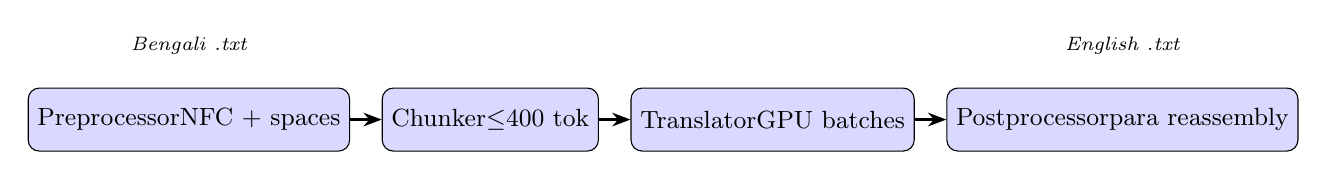
\begin{tikzpicture}[
    box/.style={rectangle, rounded corners, draw, fill=blue!15, minimum width=2.2cm, minimum height=0.8cm, font=\small},
    arrow/.style={-{Stealth}, thick},
    node distance=0.6cm and 0.4cm
  ]
    \node[box] (pre)  {Preprocessor\\NFC + spaces};
    \node[box, right=of pre] (chunk) {Chunker\\ $\le$400 tok};
    \node[box, right=of chunk] (trans) {Translator\\GPU batches};
    \node[box, right=of trans] (post)  {Postprocessor\\para reassembly};

    \draw[arrow] (pre) -- (chunk);
    \draw[arrow] (chunk) -- (trans);
    \draw[arrow] (trans) -- (post);

    \node[above=0.3cm of pre, font=\scriptsize\itshape] {Bengali .txt};
    \node[above=0.3cm of post, font=\scriptsize\itshape] {English .txt};
  \end{tikzpicture}
  \end{center}

  \begin{itemize}
    \item Chunker never splits mid-sentence (danda \texttt{।}/\texttt{॥} aware)
    \item \texttt{para\_id} metadata on each chunk drives reassembly
    \item Same paragraph count guaranteed in/out
  \end{itemize}
\end{frame}

% ── Model Zoo ───────────────────────────────────────────────────────────────
\begin{frame}{Supported Models}
  \begin{table}
  \small
  \begin{tabular}{llrrl}
    \toprule
    Key & Architecture & VRAM & FLORES BLEU & Backend \\
    \midrule
    \texttt{nllb-600M}       & M2M-100  & 2.0\,GB & 22       & CT2 float16 \\
    \texttt{nllb-1.3B}       & M2M-100  & 2.6\,GB & 26       & CT2 float16 \\
    \texttt{indicTrans2-1B}  & M2M-100v & 3.0\,GB & 44       & CT2 float16 \\
    \texttt{madlad-3b}       & T5       & 3.0\,GB & 36       & HF float16  \\
    \texttt{seamless-medium} & Custom   & 3.5\,GB & $\sim$39 & HF float16  \\
    \texttt{ollama}          & LLM      & 2.8--7.3\,GB & ---  & Ollama API  \\
    \bottomrule
  \end{tabular}
  \end{table}
  All models run \textbf{fully offline} --- no API keys required.
\end{frame}

% ── BLEU Results ────────────────────────────────────────────────────────────
\begin{frame}{Translation Quality Results}
  \begin{columns}
    \column{0.48\textwidth}
    \begin{block}{In-domain (90-sentence corpus)}
      \textbf{BLEU 65.2} overall\\
      Domain range: 4.7 (News) -- 80.6 (Health)\\
      Model: NLLB-600M CT2 float16
    \end{block}
    \vspace{0.3cm}
    \begin{block}{Open-domain (Samanantar 984 pairs)}
      BLEU 0.15 baseline\\
      BLEU 0.17 post fine-tuning\\
      (raw sacrebleu; domain mismatch expected)
    \end{block}

    \column{0.48\textwidth}
    \begin{alertblock}{Key Insight}
      Single-number BLEU masks\\
      \textbf{75-point domain variance}.\\
      Always report per-domain scores.
    \end{alertblock}
    \vspace{0.3cm}
    \begin{block}{Throughput}
      97--100\,chars/s\\
      82--84\% GPU utilisation\\
      VRAM: $\sim$1,942\,MiB
    \end{block}
  \end{columns}
\end{frame}

% ── LoRA Fine-Tuning ─────────────────────────────────────────────────────────
\begin{frame}{LoRA Fine-Tuning on RTX 5050}
  \begin{columns}
    \column{0.55\textwidth}
    \textbf{Configuration:}
    \begin{itemize}
      \item 3 epochs, 7,863 Samanantar train pairs
      \item \texttt{lora\_r=16}, \texttt{lora\_alpha=32}, \texttt{bf16=True}
      \item Batch 8, grad accum 4, lr $2\times10^{-4}$
      \item Runtime: 2.46\,h (738 steps, $\sim$12\,s/step)
    \end{itemize}
    \vspace{0.2cm}
    \textbf{Results:}
    \begin{itemize}
      \item Train loss: 9.098 $\to$ convergence
      \item Eval loss: 2.111 $\to$ 2.003 $\to$ 1.992
      \item BLEU: 0.15 $\to$ 0.17 (open-domain)
    \end{itemize}

    \column{0.4\textwidth}
    \begin{block}{Why bf16?}
      fp16 + GradScaler raises\\
      \texttt{ValueError} on sm\_120\\
      (newly discovered constraint)\\
      bf16 needs no GradScaler ---\\
      Blackwell supports it natively.
    \end{block}
  \end{columns}
\end{frame}

% ── Hardware Constraints ─────────────────────────────────────────────────────
\begin{frame}{Six Blackwell sm\_120 Deployment Constraints}
  \begin{enumerate}
    \item \textbf{INT8 cuBLAS failure} --- CT2 INT8 $\to$ \texttt{CUBLAS\_STATUS\_NOT\_SUPPORTED};
          use float16 with compute type probe
    \item \textbf{SIGBUS (misdiagnosed)} --- blamed on AMX; actual cause: corrupt pip install
    \item \textbf{Fork deadlock} --- HuggingFace fast tokenizer + CUDA fork; use \texttt{spawn}
    \item \textbf{prefetch\_factor} --- must set to 0 or 2 with CUDA DataLoader
    \item \textbf{fp16/bf16 GradScaler} --- \texttt{ValueError} when GradScaler meets fp16 on sm\_120;
          solution: \texttt{bf16=True, fp16=False}
    \item \textbf{CT2 OOM} --- translating 900+ sentences in one batch; fix: \texttt{max\_batch\_size=32}
  \end{enumerate}
  All constraints documented, root-caused, and reproducibly fixed in source.
\end{frame}

% ── Resource Monitoring ──────────────────────────────────────────────────────
\begin{frame}{Resource Monitoring Subsystem}
  \begin{itemize}
    \item \texttt{ResourceMonitor} --- daemon thread, samples CPU/RAM/GPU every 2\,s
    \item \texttt{RunDatabase} --- SQLite; every benchmark/finetune run recorded
    \item Automated regression detection and optimization recommendations
    \item CLI: \texttt{python scripts/show\_stats.py list/show/trend/compare/regressions}
  \end{itemize}
  \vspace{0.3cm}
  \begin{block}{Every run records}
    model name, BLEU score, duration, peak VRAM, avg GPU\%, input size, timestamp
  \end{block}
\end{frame}

% ── Conclusion ───────────────────────────────────────────────────────────────
\begin{frame}{Conclusion}
  \begin{itemize}
    \item \textbf{bn-en-translate}: fully offline Bengali$\to$English NMT on consumer GPU
    \item BLEU 65.2 in-domain; 97--100\,chars/s throughput on RTX 5050 (8\,GB)
    \item LoRA fine-tuning fully unlocked on Blackwell sm\_120 with bf16
    \item 5 new models added: NLLB-1.3B, IndicTrans2-1B, MADLAD-400-3B, SeamlessM4T-v2, Gemma~3
    \item Six undocumented hardware constraints resolved and documented
    \item 212 TDD tests, all passing
  \end{itemize}
  \vspace{0.4cm}
  \begin{center}
    \textbf{Open source:} \texttt{github.com/souradeepta/translate}
  \end{center}
\end{frame}

\end{document}
